\documentclass[12pt]{article}
\usepackage{amsmath}
\usepackage{amsfonts}
\usepackage{amssymb}
\usepackage{amsthm}
\usepackage[top=1in, bottom=1in, left=1in, right=1in]{geometry}
\usepackage{tikz}
\usetikzlibrary{automata,topaths,arrows}
\usepackage{caption}
\usepackage{graphicx}
\usepackage{float}
\usepackage{alltt}
\usepackage{mathrsfs}
\usepackage{ulem}
\usepackage{verbatim}

\newtheorem{theorem}{Theorem}[section]
\newtheorem{corollary}{Corollary}[theorem]

\theoremstyle{definition}
\newtheorem{defn}{Definition}[section]
\newtheorem{algorithm}{Algorithm}[section]
\newtheorem*{algorithm*}{Algorithm}

\theoremstyle{remark}
\newtheorem{remark}{Remark}[section]

\newcommand\Tau{\mathrm{T}}
\newcommand\sgn{\text{sgn}}

\newcommand{\bbR}{\mathbb{R}} %shorter commands for ``Blackboard Bold" letters
\newcommand{\bbZ}{\mathbb{Z}}
\newcommand{\bbN}{\mathbb{N}}
\newcommand{\bbC}{\mathbb{C}}
\newcommand{\bbQ}{\mathbb{Q}}
\newcommand{\bbP}{\mathbb{P}}

\newcommand{\abs}[1]{\left| #1 \right|} %shorthand absolute value
\begin{document}

Throughout this paper we will refer to a fixed regulatory network $\textnormal{\textbf{RN}} = (V,E)$ with network nodes $V = \{x_1,x_2,\dots,x_n\}$ and interactions $E \subset V \times V \times \{\rightarrow,\dashv\}$. We define the \textit{targets} of a node as
\begin{equation*}
\mathbf{T}(x_i):=\{x_j \mid (x_i,x_j) \in \mathbf{RN} \}
\end{equation*}
and the \textit{sources} of a node as 
\begin{equation*}
\mathbf{S}(x_i):=\{x_j \mid (x_j,x_i) \in \mathbf{RN} \}
\end{equation*}

\section{General System}
\begin{defn}
We define a general system of \textbf{RN} as 
\begin{equation}	\label{generalsystem}
\dot{x}_j=-\gamma_j x_j + \sum_{I\in \mathcal{I}}\left(\prod_{i\in I}\sigma_{ji}(x_i)\right)	\qquad	j=1,\dots,n
\end{equation}
where $\mathcal{I}\subseteq \mathscr{P} \{1,\dots,n\}$ and $\sigma_{ji}(x_i)$  is a linear ramp defined if $(x_i,x_j) \in E$ as
\begin{equation}	\label{sigma}
\sigma_{ji}(x_i):=
\begin{cases}
l_{ji}	&	\text{for } x_i \le \theta_{ji}-\frac{\epsilon_{ji}}{2}\ \text{and } x_i\to x_j, \text{or } x_i\geq\theta_{ji}+\frac{\epsilon_{ji}}{2} \text{ and } x_i\dashv x_j\\
u_{ji}	&	\text{for}\ x_i \geq\theta_{ji}+\frac{\epsilon_{ji}}{2}\ \text{and}\ x_i\dashv x_j, \text{or}\ x_i\le\theta_{ji}-\frac{\epsilon_{ji}}{2} \text{ and } x_i\to x_j\\
+\frac{u_{ji}-l_{ji}}{\epsilon_{ji}}(x_i-\theta_{ji}) + \frac{u_{ji}+l_{ji}}{2} &  \text{for } \theta_{ji}-\frac{\epsilon_{ji}}{2}<x_i<\theta_{ji}+\frac{\epsilon_{ji}}{2} \text{ and } x_i\to x_j\\
-\frac{u_{ji}-l_{ji}}{\epsilon_{ji}}(x_i-\theta_{ji}) + \frac{u_{ji}+l_{ji}}{2} & \text{for } \theta_{ji}-\frac{\epsilon_{ji}}{2}<x_i<\theta_{ji}+\frac{\epsilon_{ji}}{2} \text{ and } x_i\dashv x_j\\
\end{cases}
\end{equation}	
{\color{cyan} Peter: I want to add the assumptions for parameter choices here. Not really sure how to write up the formalized defintion of parameter choices as well. That remains to be done. In doing so, the next paragraph probably needs to be rewritten. Should I just borrow mostly from the parameter graph paper? Also, I don't have formal definitions for $\textnormal{\textbf{RN}}$.}
\end{defn}

The constants $u_{ji}$ and $l_{ji}$  and the thresholds $\theta_{ji}$ are as previously defined. The constants $\epsilon_{ji}$ are introduced for all $\sigma_{ji}(x_i)$ such that $\epsilon_{ji}>0$ and $\epsilon_{ji}$ is small enough to satisfy $\theta_{ki}-\frac{\epsilon_{ki}}{2},\theta_{ki}+\frac{\epsilon_{ki}}{2}\notin [\theta_{ji}-\frac{\epsilon_{ji}}{2},\theta_{ji}+\frac{\epsilon_{ji}}{2}]$ for any $i,j,k$ with $j \neq k$. That is, no epsilon bands of any single variable overlap, and so for any particular value of $x_i$, at most only one $\sigma_{ji}(x_i)$, where $x_j\in\mathbf{T}(x_i)$, is in its linear region. Therefore, we can classify intervals of $x_i$ as two distinct types.

\begin{figure}[h]	\label{sigmagraph}
\centering
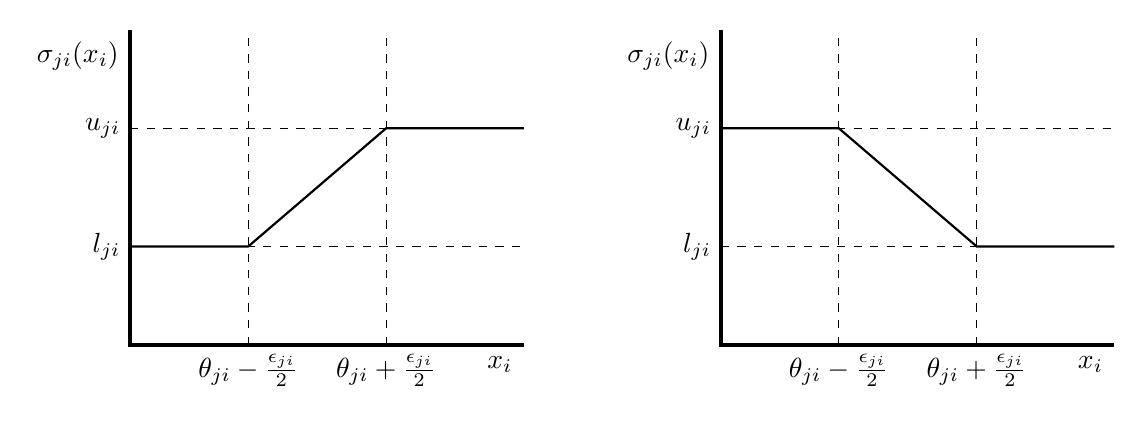
\begin{tikzpicture}[scale=1]
%\draw[step=.5cm,grey,very thin] (0,0) grid (5,4);
\draw[ultra thick] (0,4) node[anchor=north east]{$\sigma_{ji}(x_i)$} -- (0,0) -- (5,0) node[anchor=north east]{$x_i$} ;
\draw[thick] (0,1.25) -- ++(1.5,0) -- ++(1.75,1.5) -- ++(1.75,0);

\draw[dashed] (1.5,0) node [below]{$\theta_{ji}-\frac{\epsilon_{ji}}{2}$} -- ++(0,4);
\draw[dashed] (3.25,0) node [below]{$\theta_{ji}+\frac{\epsilon_{ji}}{2}$} -- ++(0,4);

\draw[dashed] (0,1.25) node[anchor=east]{$l_{ji}$} -- ++(5,0);
\draw[dashed] (0,2.75) node[anchor=east]{$u_{ji}$}-- ++(5,0);

\draw[ultra thick] (7.5,4) node[anchor=north east]{$\sigma_{ji}(x_i)$} -- (7.5,0) -- (12.5,0) node[anchor=north east]{$x_i$} ;
\draw[thick] (7.5,2.75) -- ++(1.5,0) -- ++(1.75,-1.5) -- ++(1.75,0);

\draw[dashed] (9,0) node [below]{$\theta_{ji}-\frac{\epsilon_{ji}}{2}$} -- ++(0,4);
\draw[dashed] (10.75,0) node [below]{$\theta_{ji}+\frac{\epsilon_{ji}}{2}$} -- ++(0,4);

\draw[dashed] (7.5,1.25) node[anchor=east]{$l_{ji}$} -- ++(5,0);
\draw[dashed] (7.5,2.75) node[anchor=east]{$u_{ji}$}-- ++(5,0);

\end{tikzpicture}
\caption{Left: A graph of $\sigma_{ji}(x_i)$ versus $x_i$ if $x_i \to x_j$. Right: The graph if $x_i \dashv x_j$.}
\end{figure}

\begin{defn}	\label{IntervalType}
We define a closed interval of $x_i$, denoted $I_{R,i}$, as \textit{Type R}, i.e. in a particular linear ramp region, if $\exists x_j\in\mathbf{T}(x_i)$ with associated thresholds $\theta_{ji}-\frac{\epsilon_{ji}}{2},\theta_{ji}+\frac{\epsilon_{ji}}{2}$ such that $I_{R,i}=\left[\theta_{ji}-\frac{\epsilon_{ji}}{2},\theta_{ji}+\frac{\epsilon_{ji}}{2}\right]$ for some $x_j \in \mathbf{T}(x_i)$.

Notice that for all $x_i\in V$, the associated $\sum_{I\in \mathcal{I}}\left(\prod_{i\in I}\sigma_{ji}(x_i)\right)$ is bounded above and below. Then, for each  we can choose some $c_\text{min}$


We define a closed interval of $x_i$, denoted $I_{C,i}$, as \textit{Type C} if $\exists x_q,x_r \in \mathbf{T}(x_i)$ with $q\neq r$ and $\theta_{qi}+\frac{\epsilon_{qi}}{2}<\theta_{ri}-\frac{\epsilon_{ri}}{2}$ such that $I_{c,i}:=[\theta_{qi}+\frac{\epsilon_{qi}}{2},\theta_{ri}-\frac{\epsilon_{ri}}{2}]$ or $I_{c,i}:=(-\infty,\theta_{qi}-\frac{\epsilon_{qi}}{2}]$ or $I_{c,i}:=[\theta_{ri}+\frac{\epsilon_{ri}}{2},\infty)$ and there is no Type R interval $I_{R,i}$ such that $I_{R,i}\subset I_{C,i}$. 
\end{defn}

{\color{cyan} Peter: I'd like to get rid of the infinities as endpoints of the Type C intervals. Bree mentioned something about compact metric spaces or something of the like. Could that be used?}

\begin{remark}
From Definition \ref{IntervalType}, note that every Type R interval is connected to two Type C intervals.
\end{remark}

\begin{defn} \label{kappa}
 We divide phase space into \textit{cells}, denoted $\kappa$. We define $\kappa$ as the product of the closed intervals
 \begin{equation}	\label{kappadefn}
 \kappa:=\prod_{i=1}^n I_{*,i} \quad \text{ where } \quad *=
 \begin{cases} 
 C & \text { if } i\in\alpha_c \\
 R & \text{ if } i \in \alpha_R
 \end{cases}
 \end{equation}
 where $\alpha_R$ and $\alpha_C$ partition $\{1,\dots,n\}$. We label $\kappa$ a  $m$-cell, where $m$ is the cardinality of $\alpha_R$, because in $\kappa$, there are $m$ equations of system \eqref{generalsystem} that are in their linear ramp section.

We defined two cells $\kappa$ and $\kappa'$ as adjacent if 
\begin{equation*}
\kappa:=\prod_{i=1}^n I_{*,i} \quad \text{ where } \quad *=
 \begin{cases} 
 C & \text { if } i\in\alpha_C \\
 R & \text{ if } i \in \alpha_R
 \end{cases}
 \end{equation*}
 and 
 \begin{equation*}
\kappa':=\prod_{i=1}^n I_{*',i} \quad \text{ where } \quad *'=
 \begin{cases} 
 C & \text { if } i\in\alpha_C' \\
 R & \text{ if } i \in \alpha_R'
 \end{cases}
 \end{equation*}
 where $\alpha_R$ and $\alpha_C$ partition $\{1,\dots,n\}$ and there exists some $k\in \{1,\dots,n\}$ such that $\alpha_C'=\alpha_C\setminus \{k\}$ and $\alpha_R'=\alpha_R\cup \{k\}$, and $I_{C,k}$ and $I_{R,k}$ are adjacent intervals. Then $\kappa'$ is an $(m+1)$-cell, where $m$ is the cardinality of $\alpha_R$.
 
We define the $n-1$ dimensional hyperplane $\kappa \cap \kappa'$ as the \textit{wall} between cells $\kappa$ and $\kappa'$ as the product
\begin{equation*}
\tau:=\prod_{i=1}^{k-1} I_{*,i} \times \{\vartheta_k\} \times \prod_{i=k+1}^{n} I_{*,i}
\end{equation*}
where $\vartheta_k = \theta_{jk} \pm \frac{\epsilon_{jk}}{2}$ for some $j$. We refer to $\tau$ as a wall of the $m$-cell $\kappa$.
\end{defn}

\begin{remark}
It is worth noting that all cells and walls are closed. Also, note that we use $\theta_{ji}+\frac{\epsilon_{ji}}{2}$, with two subscripts, to denote a threshold of system \eqref{generalsystem}, and $\vartheta_k$, with one subscript, to denote some constant that is the endpoint of some interval of $x_k$.
\end{remark}

%\begin{defn} \label{cornersetdefn}
%Let $\kappa$ be some cell of $\bbR^n$ with associated $\alpha_R$ and $\alpha_C$. From Definition \ref{IntervalType}, for each $i\in\alpha_R$ and corresponding $I_{R,i}$, let $r_i^+$ and $r_i^-$ be constants such that $I_{R,i}=[r_i^-,r_i^+]$, and for each $i\in\alpha_C$ and corresponding $I_{R,i}$, let $c_i^+$ and $c_i^-$ be constants such that if $I_{C,i}=[\theta_{qi}+\frac{\epsilon_{qi}}{2},\theta_{ri}-\frac{\epsilon_{ri}}{2}]$ then $I_{C,i}=[c_i^-,c_i^+]$, or {\color{cyan} Dissipative System here} . Let $P_i$ be the set defined as 
%\begin{equation} \label{cornersetequation}
%P_i :=
%\begin{cases}
%\{r_i^-,r_i^+\} &  \text{ if } i\in \alpha_R \\
%\{c_i^-,c_i^+\} &  \text{ if } i\in \alpha_C \\
%\end{cases}
%\end{equation}
%We define the set of \textit{corner points} of a cell $\kappa$, denoted $\bbP(\kappa)$, as the product of sets 
%\begin{equation*}
%\bbP (\kappa) := \prod_{i=1}^n P_i
%\end{equation*}
%Notice that the cardinality of $\bbP (\kappa)$ is $2^n$. Let $p_1,\dots,p_{2^n}$ be the elements of $\bbP (\kappa)$.
%\end{defn}

\begin{defn} \label{flowDefn}
Suppose $H$ is some subset of a co-dimension $n-1$ hyperplane with normal vector $\vec{h}$ and suppose a vector $\dot{x}(P)$ such that $\dot{x}(P)=\langle \dot{x}_1(P),\dots,\dot{x}_n(P) \rangle$ where $\dot{x}_j(P)$ denotes $\dot{x}_j$ evaluated at some point $P$. We define the \textit{flow} of system \eqref{generalsystem} to be \textit{monotonic} in the direction of $\vec{h}$ on $H$ if $\forall$ points $P$ such that $P\in H$, $\vec{h}\cdot\vec{x}(P)>0$, and monotonic in the direction of $-\vec{h}$ on $H$ if $\forall$ points $P$ such that $P\in H$, $\vec{h}\cdot\vec{x}(P)<0$. 
We define the flow to be bidirectional across $H$ if $\exists$ points $P_1,P_2$ such that $P_1,P_2 \in H$, $\vec{h}\cdot\vec{x}(P_1)>0$ and $\vec{h}\cdot\vec{x}(P_2)<0$.
\end{defn}

\begin{defn} \label{sgnDefn}
Let $A$ be any closed bounded region of $\bbR^n$, and let $P$ and $P'$ be points.  We introduce the function $\sgn(A,k)$ to classify the behavior of the solutions to system \eqref{generalsystem} in $A$, defined as 
\begin{equation}
\sgn(A,k)=
\begin{cases}
+1	&	\text{if } \forall P\in A, \dot x_k (P)>0\\
-1	&	\text{if } \forall P\in A, \dot x_k (P)<0\\
0	&	\text{if } \exists P,P'\in A \text{ such that }  \dot x_k (P)>0 \text{ and } \dot x_k (P')<0\\
\text{undefined} & \text{otherwise} \\
\end{cases}
\end{equation}
\end{defn}

\begin{remark}
From Definitions \ref{flowDefn} and \ref{sgnDefn} that if $\tau$ is some wall in $\mathbb{R}^n$ such that $\tau \subseteq \{x_k=\vartheta_k\}$, then $\sgn(\tau,k)=+1$ implies that the flow is monotonic in the $\vec e_k$ direction across $\tau$, and similarly $\sgn(\tau,k)=-1$ implies that the flow is monotonic in the $-\vec e_k$ direction across $\tau$. 
%We will occasionally use the notation $\sgn(\tau)$ to refer to $\sgn(\tau,k)$ where $\tau \subseteq \{x_k=\vartheta_k\}$. 
We will use this fact to construct the domain graph of system \eqref{generalsystem}.
\end{remark}

%{\color{cyan} Peter: The next theorem and proof is incomplete, but I'll probably leave the proof to Tomas or Bree. The Generic proof argument still escapes me.}

%\begin{theorem} \label{0cellsdefined}
%Suppose $\kappa$ is a  $0$-cell, and $\tau$ is a face of $\kappa$. It is generic that $\sgn(\tau)\neq 0$.
%\end{theorem}

%\begin{proof}
%Let $\tau\subseteq \{x_k=\vartheta_k\}$. Then $\vec{e}_k\perp \tau$ By definition of  $0$-cell, $\kappa$ is the product of n Type C intervals, and so all $\sigma_{ki}(x_i)$ are constants. The $k^\text{th}$ equation of system \eqref{generalsystem} can then be written as $\dot x_k=-\gamma_kx_k+C_k$, where $C_k$ is some constant. On $\tau$, $x_k=\vartheta_k$, and so by substitution, $\dot x_k = -\gamma_k \vartheta_k + C_k$ on $\tau$. Therefore, $\dot{x}_k=0$ only if $\gamma_k\vartheta_k=C_k$. Otherwise, $\dot{x}_k$ is some non-zero constant, and so by Definition \ref{sgnDefn}, $\sgn(\tau)\neq 0$.
%\end{proof}

%\begin{comment}
%\begin{theorem} \label{straightlineproof}
%Suppose $\kappa$ is some cell in $\mathbb{R}^n$, and suppose $\tau$ and $\tau'$ are walls of $\kappa$ such that $\tau \subseteq \{x_k=\vartheta_k\}$ and $\tau' \subseteq \{x_k=\vartheta_k'\}$ with $\vartheta'_k > \vartheta_k$. If $\sgn(\tau,i)=\sgn(\tau',i)$, %then $\sgn(\kappa,i)=\sgn(\tau,i)$.
%\end{theorem}

%\begin{proof}
%Let $Q$ be any point such that $Q\in\kappa$. Let $\alpha$ be some scalar such that $P=Q +\alpha \vec e_k $ and $P \in \tau$. Let $f(s)$ be a path such that $f:[0,1]\to\kappa$ and $f(s)$ is parameterized as $f(s)=  P + (\vartheta'-\vartheta)\vec e_ks$.  Note that then $f(0) \in \tau$ and $f(1) \in \tau'$, and that $Q\in f(s)$. If $x_k$ is not a source of $x_i$, i.e. if $x_k \notin \mathbf{S}(x_i)$, or if $k\neq i$, then $\frac{\partial}{\partial x_k}(\dot x_i)=0$, which implies that $\dot x_i$ is constant on $f(s)$, and so it follows that $\dot x_i (Q)=\dot x_i (f(0))=\dot x_i (f(1))$. However, if $x_k \in \mathbf{S}(x_i)$, then on $f(s)$, $\dot x_i$ is an affine function of $x_k$ only, and so $\frac{d}{ds}\dot x_i(f(s))$ is either $0$ or a non-zero constant, and so if $\sgn(\tau,i)=\sgn(\tau',i)=+1$, and then by Definition \ref{sgnDefn}, $\dot x_i (f(0))>0$ and $\dot x_i (f(1))>0$, and so $\dot x_i (Q))>0$, for all $Q\in f(s)$. Similarly if $\sgn(\tau,i)=\sgn(\tau',i)=-1$, then by Definition \ref{sgnDefn}, $\dot x_i (f(0))<0$ and $\dot x_i (f(1))<0$, and so $\dot x_i (Q))<0$ for all $Q\in f(s)$. Since $Q$ was arbitrary the result follows by Definition \ref{sgnDefn}.
%\end{proof}

\begin{defn}
Let $A$ be a closed region of $\bbR^n$ such that $A:=\prod^{n}_{i=1}a_i$ where 
\begin{equation*}
a_i =
\begin{cases}
I_{C,i} & \text{if } i\in\alpha_C\\
I_{R,i} & \text{if } i\in\alpha_R\\
\{f_i\} & \text{otherwise}
\end{cases}
\end{equation*}
and $\alpha_C$ and $\alpha_R$ partition some subset of $\{1,\dots,n\}$, $I_{C,i}$ is some Type C interval of $x_i$, $I_{R,i}$ is some Type R interval of $x_i$, and $f_i$ is any arbitrary constant. For each $i\in\alpha_C$, let $c_i^+$ and $c_i^-$ be the endpoints of $I_{C,i}$ such that $I_{C,i}=[c_i^-,c_i^+]$, and for each $i\in\alpha_R$, let $r_i^+$ and $r_i^-$ be the endpoints of $I_{R,i}$ such that $I_{R,i}=[r_i^-,r_i^+]$. We define the set of \textit{corner points} of $A$ as $\bbP(A)$, where
\begin{equation*}
\bbP(A):=\prod_{i=1}^n P_i \quad \text{where} \quad P_i=\begin{cases}
\{c_i^-,c_i^+\} & \text{if } i\in\alpha_C \\
\{r_i^-,r_i^+\} & \text{if } i\in\alpha_R \\
\{f_i\} & \text{otherwise}
\end{cases}
\end{equation*}
\end{defn}

\begin{theorem} \label{straightlineproof}
Suppose $A$ be a closed region of $\bbR^n$ with associated $\alpha_C$ and $\alpha_R$, and suppose $\alpha_C \cup \alpha_R \neq \emptyset$. For some $k\in \alpha_C \cup \alpha_R$, let $I_{*,k}$ be the associated interval, and let $\vartheta_k$ and $\vartheta_k'$ be the endpoints of $I_{*,k}$ such that $I_{*,k}=[\vartheta_k,\vartheta_k']$. Let $W:=A\cap \{x_k=\vartheta_k\}$ and let $W':=A\cap \{x_k=\vartheta_k'\}$. If $\sgn(W,j)=\sgn(W',j)\neq 0$, then $\sgn(W,j)=\sgn(A,j)$.
\end{theorem}

\begin{proof}
Suppose $Q$ is any point such that $Q\in A$. Then there exists some scalar $\beta\geq 0$ such that $Q-\beta \vec e_k\in W$. Let $f:[0,1]\to A$ be a function such that $f(s)=(Q-\beta \vec e_k) + s(\vartheta_k'=\vartheta_k) \vec e_k$ for $0\leq s \leq 1$. Note that $f(0)\in W$ and $f(0)\in W'$. Also note that from system \eqref{generalsystem}, $\dot x_j$ is an affine function of only $x_k$ on $f(s)$. Recall from Definition \ref{sgnDefn}, if $\sgn(W,j)=\sgn(W',j)=+1$, then $\dot x_j (f(0))>0$ and $\dot x_j (f(1))>0$. It follows that for all $s^*\in [0,1]$, $\dot x_j (f(s^*))>0$, and so  $\dot x_j (Q))>0$. As $Q$ was arbitrary, then from Definition \ref{sgnDefn}, $\sgn(A,j)=\sgn(W,j)$. A similar argument is used when $\sgn(W,j)=\sgn(W',j)=-1$.
\end{proof}

\begin{theorem} \label{cornerpointproof}
Let $A$ be a closed region of $\bbR^n$ with associated $\alpha_C$ and $\alpha_R$. If and only if for all $p\in\bbP(A)$, $\sgn(p,j)$ is defined and the same, then $\sgn(A,j)=\sgn(p_1,j)$.
\end{theorem}

\begin{proof}
First we will show the converse direction. Suppose $\sgn(A,j)=\sgn(p_1,j)$. Note that for a single point $p_1$, $\sgn(p_1,j)\neq 0$, and so $\sgn(A,j)\neq 0$, and the proof is immediate from Definition \ref{sgnDefn}.

Now we will show the forward direction. Suppose $n=1$. If $1\notin \alpha_C \cup \alpha_R$, then $A=\{f_1\}$, and therefore $A=\bbP(A)$ and $\sgn(A,1)=\sgn(p_1,1)$. However, if $1\in \alpha_C \cup \alpha_R$, then $A=I_{*,1}=[\vartheta_1,\vartheta_1']$. Let $W=\{\vartheta_1\}$ and $W'=\{\vartheta'_1\}$. Note that $\bbP(A)=\{W,W'\}$, and so by Theorem \ref{straightlineproof} the theorem holds.

Now assume for all $n$-dimensional systems in the form of \eqref{generalsystem} the theorem holds. Consider any $(n+1)$-dimensional system in the form of \eqref{generalsystem}. Let $A$ be a closed region of $\bbR^{(n+1)}$ with associated $\alpha_C$ and $\alpha_R$, and suppose for all $p\in\bbP(A)$, $\sgn(p,j)$ is defined and the same. If $\alpha_C \cup \alpha_R=\emptyset$, then $A$ is a single point and the proof is immediate. If $\alpha_C \cup \alpha_R \neq \emptyset$, then we can find some $k\in \alpha_C \cup \alpha_R$. Let $I_{*,k}$ be the associated interval of $A$ with endpoints $\vartheta_k$ and $\vartheta_k'$. Let $W=A \cap \{x_k=\vartheta_k\}$ and $W'=A \cap \{x_k=\vartheta_k'\}$. Notice that on the hyperplane $\{x_k=\vartheta_k\}$, the system reduces to an $n$-dimensional system. Also note that $\bbP(W)\subseteq\bbP(A)$, and so by assumption $\sgn(W,j)=\sgn(p_1,j)$. By a similar argument $\sgn(W',j)=\sgn(p_1,j)$. Then by Theorem \ref{straightlineproof}, $\sgn(A,j)=\sgn(W',j)=\sgn(p_1,j)$ and the theorem holds. 
\end{proof} 


\begin{remark} \label{cornerpointsin0cell}
We apply Theorem \ref{cornerpointproof} to the walls and cells of $\textnormal{\textbf{RN}}$. Given any wall, we can now unambiguously determine the flow through the wall if we know the $\sgn$ of all corner points of that wall. Notice that for all $i\in\alpha_R$, $I_{R,i}=[r_i^-,r_i^+]$, and recall that every Type R interval is connected to two Type C intervals and all intervals are closed, and so there must exists two Type C intervals $I_{C,i}$ and $I_{C,i}'$ such that $r_i^-\in I_{C,i}$ and  $r_i^+\in I_{C,i}'$. Then it follows that for each point $p\in\bbP(\kappa)$, there exists some $0$-cell $\kappa^*$, and some wall $\tau^*$ of $\kappa^*$ such that $p\in\tau^*$. 

Furthermore, note that for any wall $\tau$, if $\tau$ is a wall of some cell $\kappa$, then $\bbP(\tau)\subset \bbP(\kappa)$, and so all points in $\bbP(\tau)$ are also contained in the wall of a zero cell. By our assumptions, all walls of zero cells have defined, non-zero $\sgn$. We use this fact to unambiguously determine the flow through all walls of $\textnormal{\textbf{RN}}$, and then to construct the domain graph of $\textnormal{\textbf{RN}}$.
\end{remark}

\section{Algorithm}

\begin{defn}
Suppose $\tau$ is some wall of an $m$-cell where $m\neq 0$, with associated $\alpha_C$ and $\alpha_R$. Let $\bbP (\tau)$ be the associated set of corner points. We define the \textit{reduced set of corner points}, denoted $\bar \bbP (\tau)$ as $
\bar \bbP (\kappa) := \prod_{i=1}^n \bar P_i$,
where $\bar P_i$ is the set defined as defined as
\begin{equation*}
\bar P_i :=
\begin{cases}
\{r_i^-,r_i^+\} &  \text{ if } i\in \alpha_R \\
\{c_i^*\} &  \text{ if } i\in \alpha_C \\
\end{cases}
\end{equation*}
where $c^*_i$ is an arbitrary value chosen such that $c^*_i \in I_{C,i}$. Note that the cardinality  $\bar \bbP (\tau)$ is $2^m$, where $m$ is the cardinality of $\alpha_R$.  Let $\bar p_i$ be a component of $\bar \bbP (\tau)$.
\end{defn}

\begin{algorithm*}
For each wall $\tau$ of an $m$-cell where $m\neq 0$ and $\tau \subseteq \{x_k=\vartheta_k\}$, let $\bbP (\tau)$ be the associated set of corner points, and let $\bar \bbP (\tau)$ be the reduced set of corner points. For each $\bar p_i \in  \bar \bbP (\tau)$, let $S_i := \sgn(\bar p_i, k)$. 
\begin{equation} \label{algorithmequation}
\text{If } \abs{\sum_{i=1}^{2^m}S_i}<\sum_{i=1}^{2^m} \abs{S_i},\text{ then }\sgn(\tau,k)=0;\text{ otherwise }\sgn(\tau,k)=S_1.
\end{equation}
\end{algorithm*}
\end{document}
